%%%%%%%%%%%%%%%%%%%%%%%%%%%%%%%%%%%%%%%%%%%%%%%%%%%%%%%%%%%%%%%%%%
\section{Mantle: A Programmable Metadata Load Balancer}
\label{mantle-implementation}							%%%%%%%%%%
%%%%%%%%%%%%%%%%%%%%%%%%%%%%%%%%%%%%%%%%%%%%%%%%%%%%%%%%%%%%%%%%%%
\begin{figure*}
	\centering
	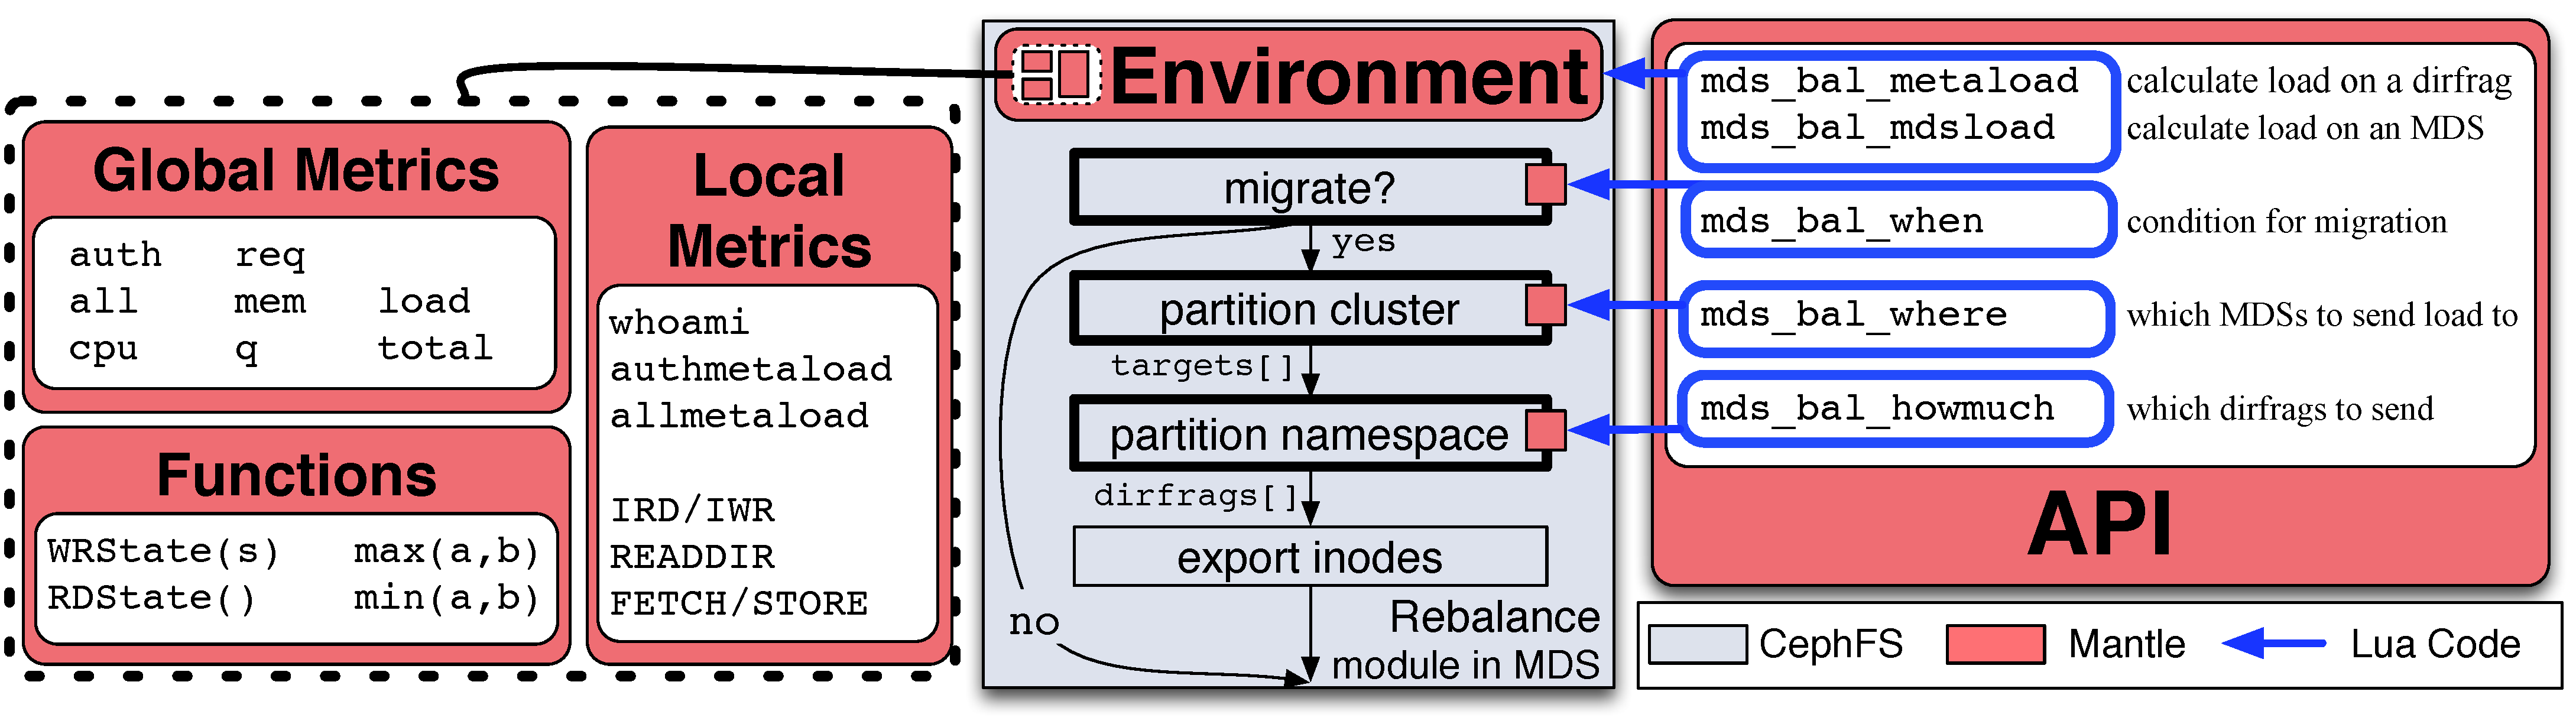
\includegraphics[width=1\textwidth]{./chapters/mantle/figures/balancer-api.pdf} 
	\caption{Designers set policies using the Mantle API. The injectable code uses the metrics/functions in the environment. \label{figure:balancer-api}}  
\end{figure*}

% why we can poke holes
The CephFS policies shape the decision making to be decentralized, aggressive, fast, and slightly forgetful. While these policies work for some workloads, including the workloads used to benchmark CephFS~\cite{weil:sc2004-dyn-metadata}, they do not work for others (as demonstrated in Figure~\ref{figure:creates-thruput}), they underutilize MDS nodes by spreading load to all MDS nodes even if the job could be finished with a subset, they destroy locality by distributing metadata without considering the workload, and they make it harder to coalesce the metadata back to one server after the flash crowd. We emphasize that the problem is that the policies are hardwired into the system, not the policies themselves. 

% Benefits of decoupling
Decoupling the policies from the mechanisms has many advantages: it gives future designers the flexibility to explore the trade-offs of different policies without fear of breaking the system, it keeps the robustness of well-understood implementations intact when exploring new policies, and it allows policies to evolve with new technologies and hardware. For example, McKusick~\cite{mckusick:fast2015-FFS} made the observation that when designing the block allocation mechanism in the Fast File System (FFS), decoupling policy from mechanism greatly enhanced the usability, efficiency, and effectiveness of the system. The low-level allocation mechanism in the FFS has not changed since 1982, but now the developer can try many different policies, even the worst policy imaginable, and the mechanism will never curdle the file system, by doing things like double allocating. 

% What we retained:
Mantle builds on the implementations and data structures in the CephFS balancer, as shown in Figure~\ref{figure:balancer-api}. The mechanisms for dynamic subtree partitioning, including directory fragmentation, moving inodes from one MDS to another, and the exchange of heartbeats, are left unmodified. While this is a standard technique, applying it to a new problem can still be novel, particularly where nobody previously realized they were separable or has tried to separate them.

%%%%%%%%%%%%%%%%%%%%
\subsection{The Mantle Environment}
\label{the-mantle-environment}
%%%%%%%%%%%%%%%%%%%%
\begin{table}[tb]
	\centering
	\ssp
	\begin{tabular}{ >{}p{4cm} | >{}p{10cm}}
    	\centering Current MDS metrics
		& \centering Description
		\tabularnewline\hline	
		\small\texttt{whoami}
		& current MDS 
		\tabularnewline
		\small\texttt{authmetaload}
		& metadata load on authority subtree
		\tabularnewline	        
		\small\texttt{allmetaload}
		& metadata load on all subtrees
		\tabularnewline	     
		\small\texttt{IRD,IWR}
		& \# inode reads/writes (with a decay)
		\tabularnewline
		\small\texttt{READDIR,FETCH,STORE}
		& \# read directories, fetches, stores
		\tabularnewline	                
        \multicolumn{2}{c}{}
        \tabularnewline
       
		\centering Metrics on MDS {\it i}
		& \centering Description
		\tabularnewline\hline       
		\small\texttt{MDSs[i]["auth"]}	
		& metadata load on authority subtree
		\tabularnewline			
		\small\texttt{MDSs[i]["all"]}	
		& metadata load on all subtrees
		\tabularnewline	        
		\small\texttt{MDSs[i]["cpu"]}
		& \% of total CPU utilization
		\tabularnewline	
		\small\texttt{MDSs[i]["mem"]}	
		& \% of memory utilization
		\tabularnewline	
		\small\texttt{MDSs[i]["q"]}	
		& \# of requests in queue
		\tabularnewline
		\small\texttt{MDSs[i]["req"]}	
		& request rate, in req/sec
		\tabularnewline				
		\small\texttt{MDSs[i]["load"]}	
		& result of \texttt{mds\_bal\_mdsload}
        \tabularnewline
		\small\texttt{total}
		& sum of the load on each MDS        
        \tabularnewline
        \multicolumn{2}{c}{}
        \tabularnewline
        
		\centering Global Functions
		& \centering Description
		\tabularnewline\hline	 
		\small\texttt{WRstate(s)}
		& save state \texttt{s}
        \tabularnewline
        \small\texttt{RDstate()}	
		& read state left by previous decision
        \tabularnewline
        \small\texttt{max(a,b),min(a,b)}
        & get the max, min of two numbers
	\end{tabular}
	\dsp
	\caption{The Mantle environment.\label{table:metrics}}    
\end{table}
Mantle decouples policy from mechanism by letting the designer inject code to control 4 policies: load calculation, ``when" to move load, ``where" to send load, and the accuracy of the decisions. Mantle balancers are written in Lua because Lua is fast (the LuaJIT virtual machine achieves near native performance) and it runs well as modules in other languages~\cite{grawinkel:pdsw2012-lua}. We could have used C but Lua gives administrators a simple syntax for writing short, storage-agnostic code that can be changed dynamically. The balancing policies are injected at run time with Ceph's command line tool, {\it e.g.,} \texttt{\small ceph tell mds.0 injectargs mds\_bal\_metaload IWR}. This command means ``tell MDS 0 to calculate load on a dirfrag by the number of inode writes".

% Global variables
Mantle provides a general environment with global variables and functions, shown on the left side of Figure~\ref{figure:balancer-api}, that injectable code can use. Local metrics are the current values for the metadata loads and are usually used to account for the difference between the stale global load and the local load. The library extracts the per-MDS metrics from the MDS heartbeats and puts the global metrics into an MDSs array. The injected code accesses the metric for MDS {\it i} using MDSs[i][``metric"]. The metrics and functions are described in detail in Table~\ref{table:metrics}. The labeled arrows between the phases in Figure~\ref{figure:balancer-api} are the inputs and outputs to the phases; inputs can be used and outputs must be filled by the end of the phase.

% WR/ReadState
The \texttt{WRstate} and \texttt{RDstate} functions help the balancer ``remember'' decisions from the past. For example, in one of the balancers, we wanted to make migration decisions more conservative, so we used \texttt{WRstate} and \texttt{RDstate} to trigger migrations only if the MDS is overloaded for 3 straight iterations. These are implemented using temporary files but future work will store them in RADOS objects to improve scalability.

%%%%%%%%%%%%%%%%%%%%
\subsection{The Mantle API}
\label{the-mantle-api}
%%%%%%%%%%%%%%%%%%%%
% What we did
Figure~\ref{figure:balancer-api} shows where the injected code fits into CephFS: the load calculations and ``when'' code is used in the ``migrate?" decision, the ``where'' decision is used when partitioning the cluster, and the ``howmuch'' decision is used when partitioning the namespace for deciding the accuracy of sending dirfrags. To introduce the API we use the original CephFS balancer as an example. 

\textbf{Metadata/MDS Loads}: these load calculations quantify the work on a subtree/dirfrag and MDS. Mantle runs these calculations and stuffs the results in the \texttt{auth}/\texttt{all} and \texttt{load} variables of Table~\ref{table:metrics}, respectively. To mimic the scalarizations in the original CephFS balancer, one would set \texttt{mds\_} \texttt{bal\_}\texttt{metaload} to:

{\small\begin{verbatim}
IRD + 2*IWR + READDIR + 2*FETCH + 4*STORE
\end{verbatim}}

\noindent and \texttt{mds\_bal\_mdsload} to:

{\small\begin{verbatim}
0.8*MDSs[i]["auth"] + 0.2*MDSs[i]["all"]
+ MDSs[i]["req"] + 10*MDSs[i]["q"]
\end{verbatim}}

The metadata load calculation values inode reads (IRD) less than the writes (IWR), fetches and stores, and the MDS load emphasizes the queue length as a signal that the MDS is overloaded, more than the request rate and metadata loads. 

\textbf{When}: this hook is specified as an ``if'' statement. If the condition evaluates to true, then migration decisions will be made and inodes may be migrated. If the condition is false, then the balancer exits immediately. To implement the original balancer, set \texttt{mds\_bal\_when} to:

{\small\begin{verbatim}
if MDSs[whoami]["load"] > total/#MDSs then
\end{verbatim}}

This forces the MDS to migrate inodes if the load on itself is larger than the average cluster load. This policy is dynamic because it will continually shed load if it senses cluster imbalance, but it also has the potential to thrash load around the cluster if the balancer makes poor decisions. 

\textbf{Where}: the designer specifies where to send load by populating the \texttt{targets} array. The index is the MDS number and the value is set to how much load to send. For example, to send off half the load to the next server, round robin, set \texttt{mds\_bal\_where} to:

{\small\begin{verbatim}
targets[i] = MDSs[whoami + 1]["load"]/2
\end{verbatim}}

The user can also inject large pieces of code. The original CephFS ``where'' balancer can be implemented in 20 lines of Lua code (not shown). 

\textbf{How Much}: recall that the original balancer sheds load by traversing down the namespace and shedding load until reaching the target load for each of the remote MDS nodes. Mantle traverses the namespace in the same way, but exposes the policy for how much to move at each level. Every time Mantle considers a list of dirfrags or subtrees in a directory, it transfers control to an external Lua file with a list of strategies called dirfrag selectors. The dirfrag selectors choose the dirfrags to ship to a remote MDS, given the target load. The ``howmuch" injectable argument accepts a list of dirfrag selectors and the balancer runs all the strategies, selecting the dirfrag selector that gets closest to the target load. We list some of the Mantle example dirfrag selectors below:
\begin{enumerate}\itemsep -2pt
%	\item send biggest dirfrags: \hfill MDS0=66.5, MDS1= 44.7
%	\item send biggest + 1: \hfill MDS0=52.8, MDS1= 58.4	
%	\item send smallest dirfrags: \hfill MDS0=58.4, MDS1= 52.8
%	\item send smallest + 1: \hfill MDS0=44.7, MDS1= 66.5	
%	\item alternate big/small: \hfill MDS0=68.4, MDS1= 42.8	
%	\item alternate big/small + 1: \hfill MDS0=55.1, MDS1= 56.1		
	\item \texttt{big\_first}: biggest dirfrags until reaching target
%	\item[] {\tiny\(15.5+14.6+14.6+13.7\) \hfill MDS0=66.5, MDS1= 44.7}
	\item \texttt{small\_first}: smallest dirfrags until reaching target
%	\item[] {\tiny\(12.7+13.3+13.3+13.5+13.7\)\hfill MDS0=44.7, MDS1= 66.5}
	\item \texttt{big\_small}: alternate sending big and small dirfrags
%	\item[] {\tiny\(15.5+12.7+14.6+13.3\) \hfill MDS0=55.1, MDS1= 56.1}
	\item \texttt{half}: send the first half of the dirfrags
%	\item[] {\tiny\(12.7+13.3+13.3+14.6\) \hfill MDS0=57.3, MDS1= 53.9}
\end{enumerate}
If these dirfrag selectors were running for the problematic dirfrag loads in Section~\S\ref{the-cephfs-policies} (12.7, 13.3, 13.3, 14.6, 15.7, 13.5, 13.7, 14.6),  Mantle would choose the \texttt{big\_small} dirfrag selector because the distance between the target load (55.6) and the load actually shipped is the smallest (0.5). To use the same strategy as the original balancer, set \texttt{mds\_bal\_how\-much} to: \texttt{\{"big\_first"\}}

% Explain that we don't control the actual selection of the subtrees
This hook does not control which subtrees are actually selected during namespace traversal ({\it i.e.} ``which part"). Letting the administrator select specific directories would not scale with the namespace and could be achieved with separate mount points. Mantle uses one approach for traversing the namespace because starting at the root and drilling down into directories ensures the highest spatial and temporal locality, since subtrees are divided and migrated only if their ancestors are too popular to migrate. Policies that influence decisions for dividing, coalescing, or migrating specific subtrees based on other types of locality ({\it e.g.,} request type) are left as future work.

\subsection{Mantle on Programmable Storage}
\label{sec:mantle-progstorage}

The original implementation is ``hard-coded" into Ceph and lacked robustness
(no versioning, durability, or policy distribution).  Re-implemented using
Malacology, Mantle now enjoys (1) the versioning provided by Ceph's monitor
daemons and (2) the durability and distribution provided by Ceph's reliable
object store.  Re-using the internal abstractions with Malacology resulted in a
2\(\times\) reduction in source code compared to the original implementation.

\subsubsection{Versioning Balancer Policies}

Ensuring that the version of the current load balancer is consistent across the
physical servers in the metadata cluster was not addressed in the original
implementation. The user had to set the version on each individual server and
it was trivial to make the versions inconsistent. Maintaining consistent
versions is important for cooperative balancing policies, where local decisions
are made assuming properties about other instances in the cluster.

With Malacology, Mantle stores the version of the current load balancer in the
Service Metadata interface. The version of the load balancer corresponds to an
object name in the balancing policy. Using the Service Metadata interface means
Mantle inherits the consistency of Ceph's internal monitor daemons. The user
changes the version of the load balancer using a new CLI command.

\subsubsection{Making Balancer Policies Durable}

The load balancer version described above corresponds to the name of an object
in RADOS that holds the actual Lua balancing code.  When metadata server nodes
start balancing load, they first check the latest version from the metadata
server map and compare it to the balancer they have loaded. If the version has
changed, they dereference the pointer to the balancer version by reading the
corresponding object in RADOS. This is in contrast to the original Mantle
implementation which stored load balancer code on the local file system -- a
technique which is unreliable and may result in silent corruption.

The balancer pulls the Lua code from RADOS synchronously; asynchronous reads
are not possible because of the architecture of the metadata server. The
synchronous behavior is not the default behavior for RADOS operations, so we
achieve this with a timeout: if the asynchronous read does not come back within
half the balancing tick interval the operation is canceled and a Connection
Timeout error is returned. By default, the balancing tick interval is 10
seconds, so Mantle will use a 5 second timeout.

This design allows Mantle to immediately return an error if anything
RADOS-related goes wrong.  We use this implementation because we do not want to
do a blocking object storage daemon read from inside the global metadata server
lock. Doing so would bring down the metadata server cluster if any of the
object storage daemons are not responsive.

Storing the balancers in RADOS is simplified by the use of an interpreted
language for writing balancer code. If we used a language that needs to be
compiled, like the C++ object classes in the object storage daemon, we would
need to ensure binary compatibility, which is complicated by different
operating systems, distributions, and compilers.

\subsubsection{Logging, Debugging, and Warnings}

In the original implementation, Mantle would log all errors, warnings, and
debug messages to a log stored locally on each metadata server. To get the
simplest status messages or to debug problems, the user would have to log into
each metadata server individually, look at the logs, and reason about causality
and ordering.

With Malacology, Mantle re-uses the centralized logging features of the
monitoring service. Important errors, warnings, and info messages are collected
by the monitoring subsystem and appear in the monitor cluster log so instead of
users going to each node, they can watch messages appear at the monitor daemon.
Messages are logged sparingly, so as not to overload the monitor with frivolous
debugging but important events, like balancer version changes or failed
subsystems, show up in the centralized log.

